\label{appendix:projection_derivation}
\section{$Proj(\theta,y)$ Derivation}

In this section, the projection operator will be defined.  Adaptive controllers often use the projection operator in their adaptive laws to ensure uniform boundedness of the system error.  This can aid in faster adaptation and ensure controller closed-loop stability.  The projection operator attempts to mathematically achieve two objectives; ensure the Lyapunov function time derivative remains negative semi-definite, and to keep the estimated parameters uniformly bounded.  Using the projection operator ensures that $\theta$ is locally Lipchitz continuous even though the input $y$ is piecewise continuous.  The projection operator as utilized in this research is defined as:

\begin{equation}
Proj(\theta,y)\triangleq 	
	\begin{cases}
	y& \text{if }f(\theta)>0, \\
	y& \text{if }f(\theta) \leq 0\text{ and }\nabla f^\top y\geq 0,\\
	y-\frac{\nabla f}{\|\nabla f\|}\left\langle\frac{\nabla f}{\|\nabla f\|},y\right\rangle f(\theta)& \text{if }f(\theta)\leq 0\text{ and }\nabla f^\top y< 0.
	\end{cases}	
\end{equation}

where $\epsilon>0$,
\begin{equation}\label{eq:parabolic_operator}
	f(\theta)=-\frac{\theta^2-\theta_{\text{max}}^2}{\epsilon \theta_{\text{max}}^2}\\
\end{equation}
\begin{equation}
	\nabla f^\top=-\frac{2\theta}{\epsilon \theta_{\text{max}}^2}
\end{equation}

The projection function chosen for this research is parabolic and has inflection points at user defined maximum/minimum bands.  Equation~\ref{eq:parabolic_operator} is plotted in figure~\ref{fig:projection_operator} with example maximum/minimum of $0.65$ and various values for $\epsilon$.  The engineer must set the value for $\epsilon$ to achieve the desired slope of the projection at the maximum values.  This slope should be steep enough to capture the highest expected error given one recursion through the algorithm.
\begin{figure}[h!]
 \centering
  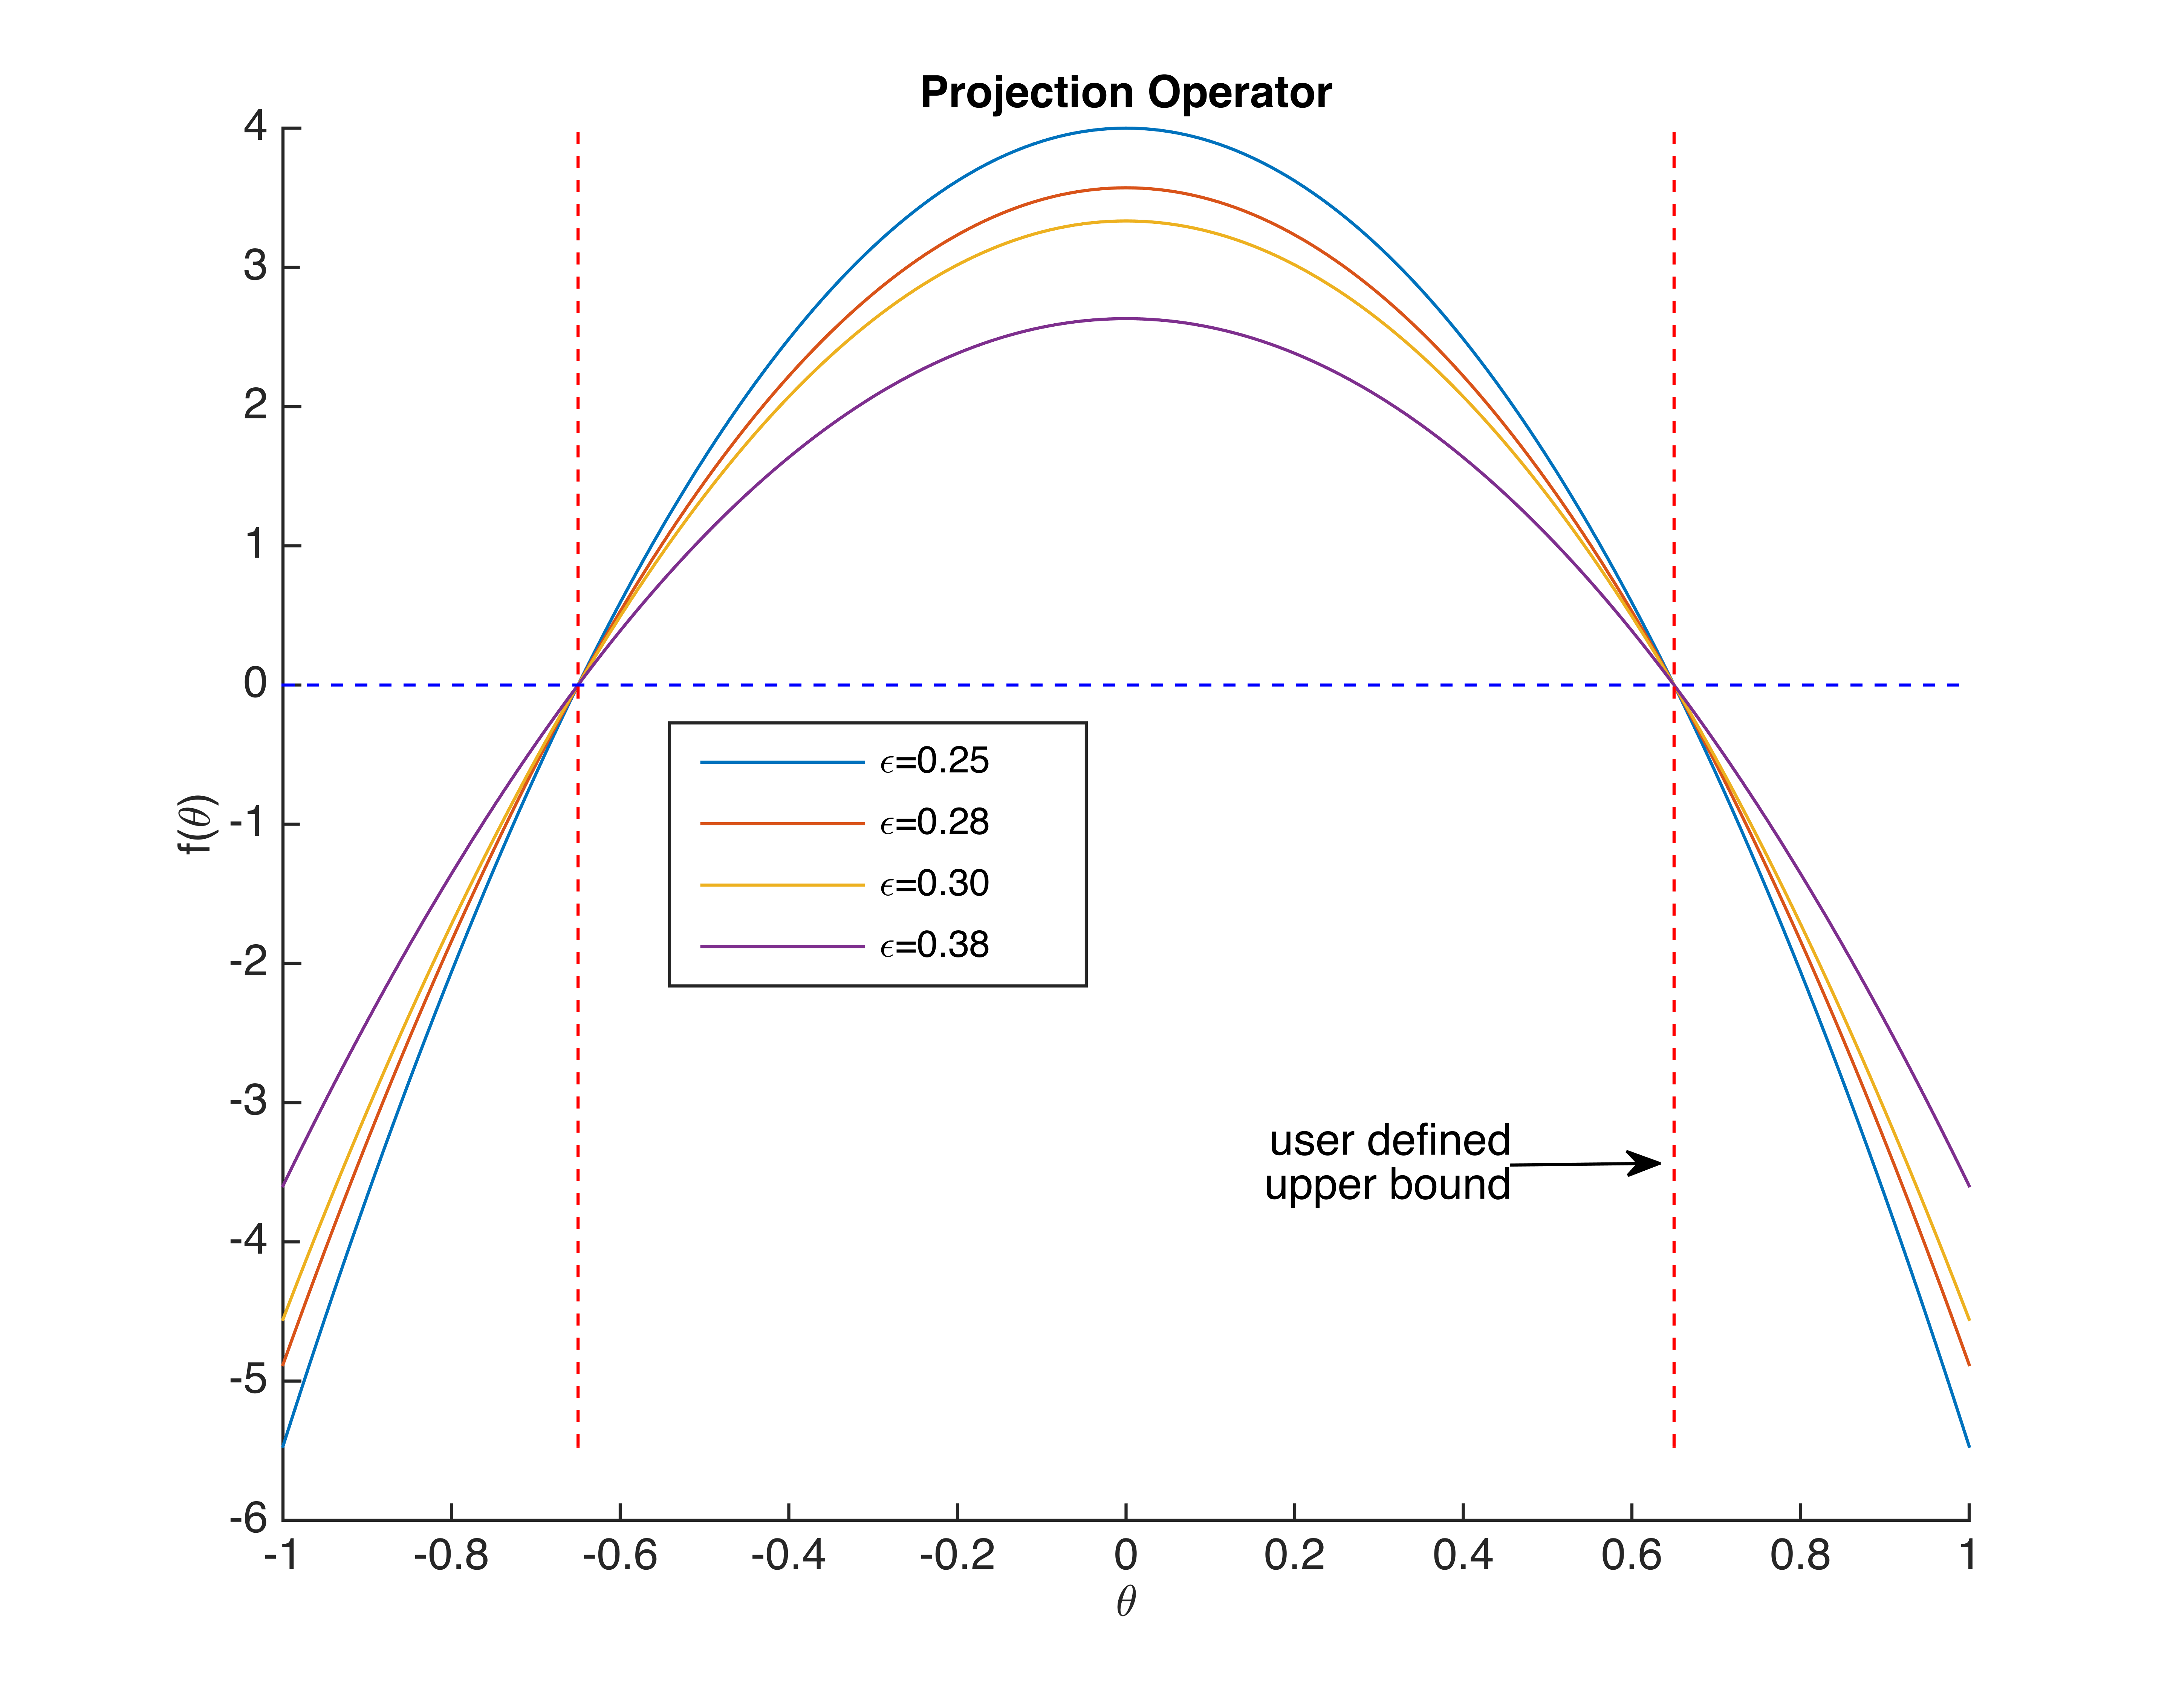
\includegraphics[width=1\textwidth]{Projection_Operator.png}
  \caption{Projection Operator - $f(\theta)$}
  \label{fig:projection_operator}
\end{figure}

There may exists systems which need to have projection bounds which are not symmetrical about zero.  This was found to be the case for this research and therefore the following projection function was used to assist the engineer tuning the algorithm:\newline
\newline
where $\epsilon>0$,
\begin{equation}\label{eq:parabolic_operator_offset}
	f(\theta)=-\frac{4(\theta_{\text{min}}-\theta)(\theta_{\text{max}}-\theta)}{\epsilon(\theta_{\text{max}}-\theta_{\text{min}})^2}\\
\end{equation}
\begin{equation}
	\nabla f^\top=\frac{4(\theta_{\text{min}}+\theta_{\text{max}}-2\theta)}{\epsilon(\theta_{\text{max}}-\theta_{\text{min}})^2}
\end{equation}


Equation~\ref{eq:parabolic_operator_offset} is plotted in figure~\ref{fig:projection_operator_offset} with example maximum of $0.65$, minimum of $0.25$,  and various values for $\epsilon$. 
\begin{figure}[h!]
 \centering
  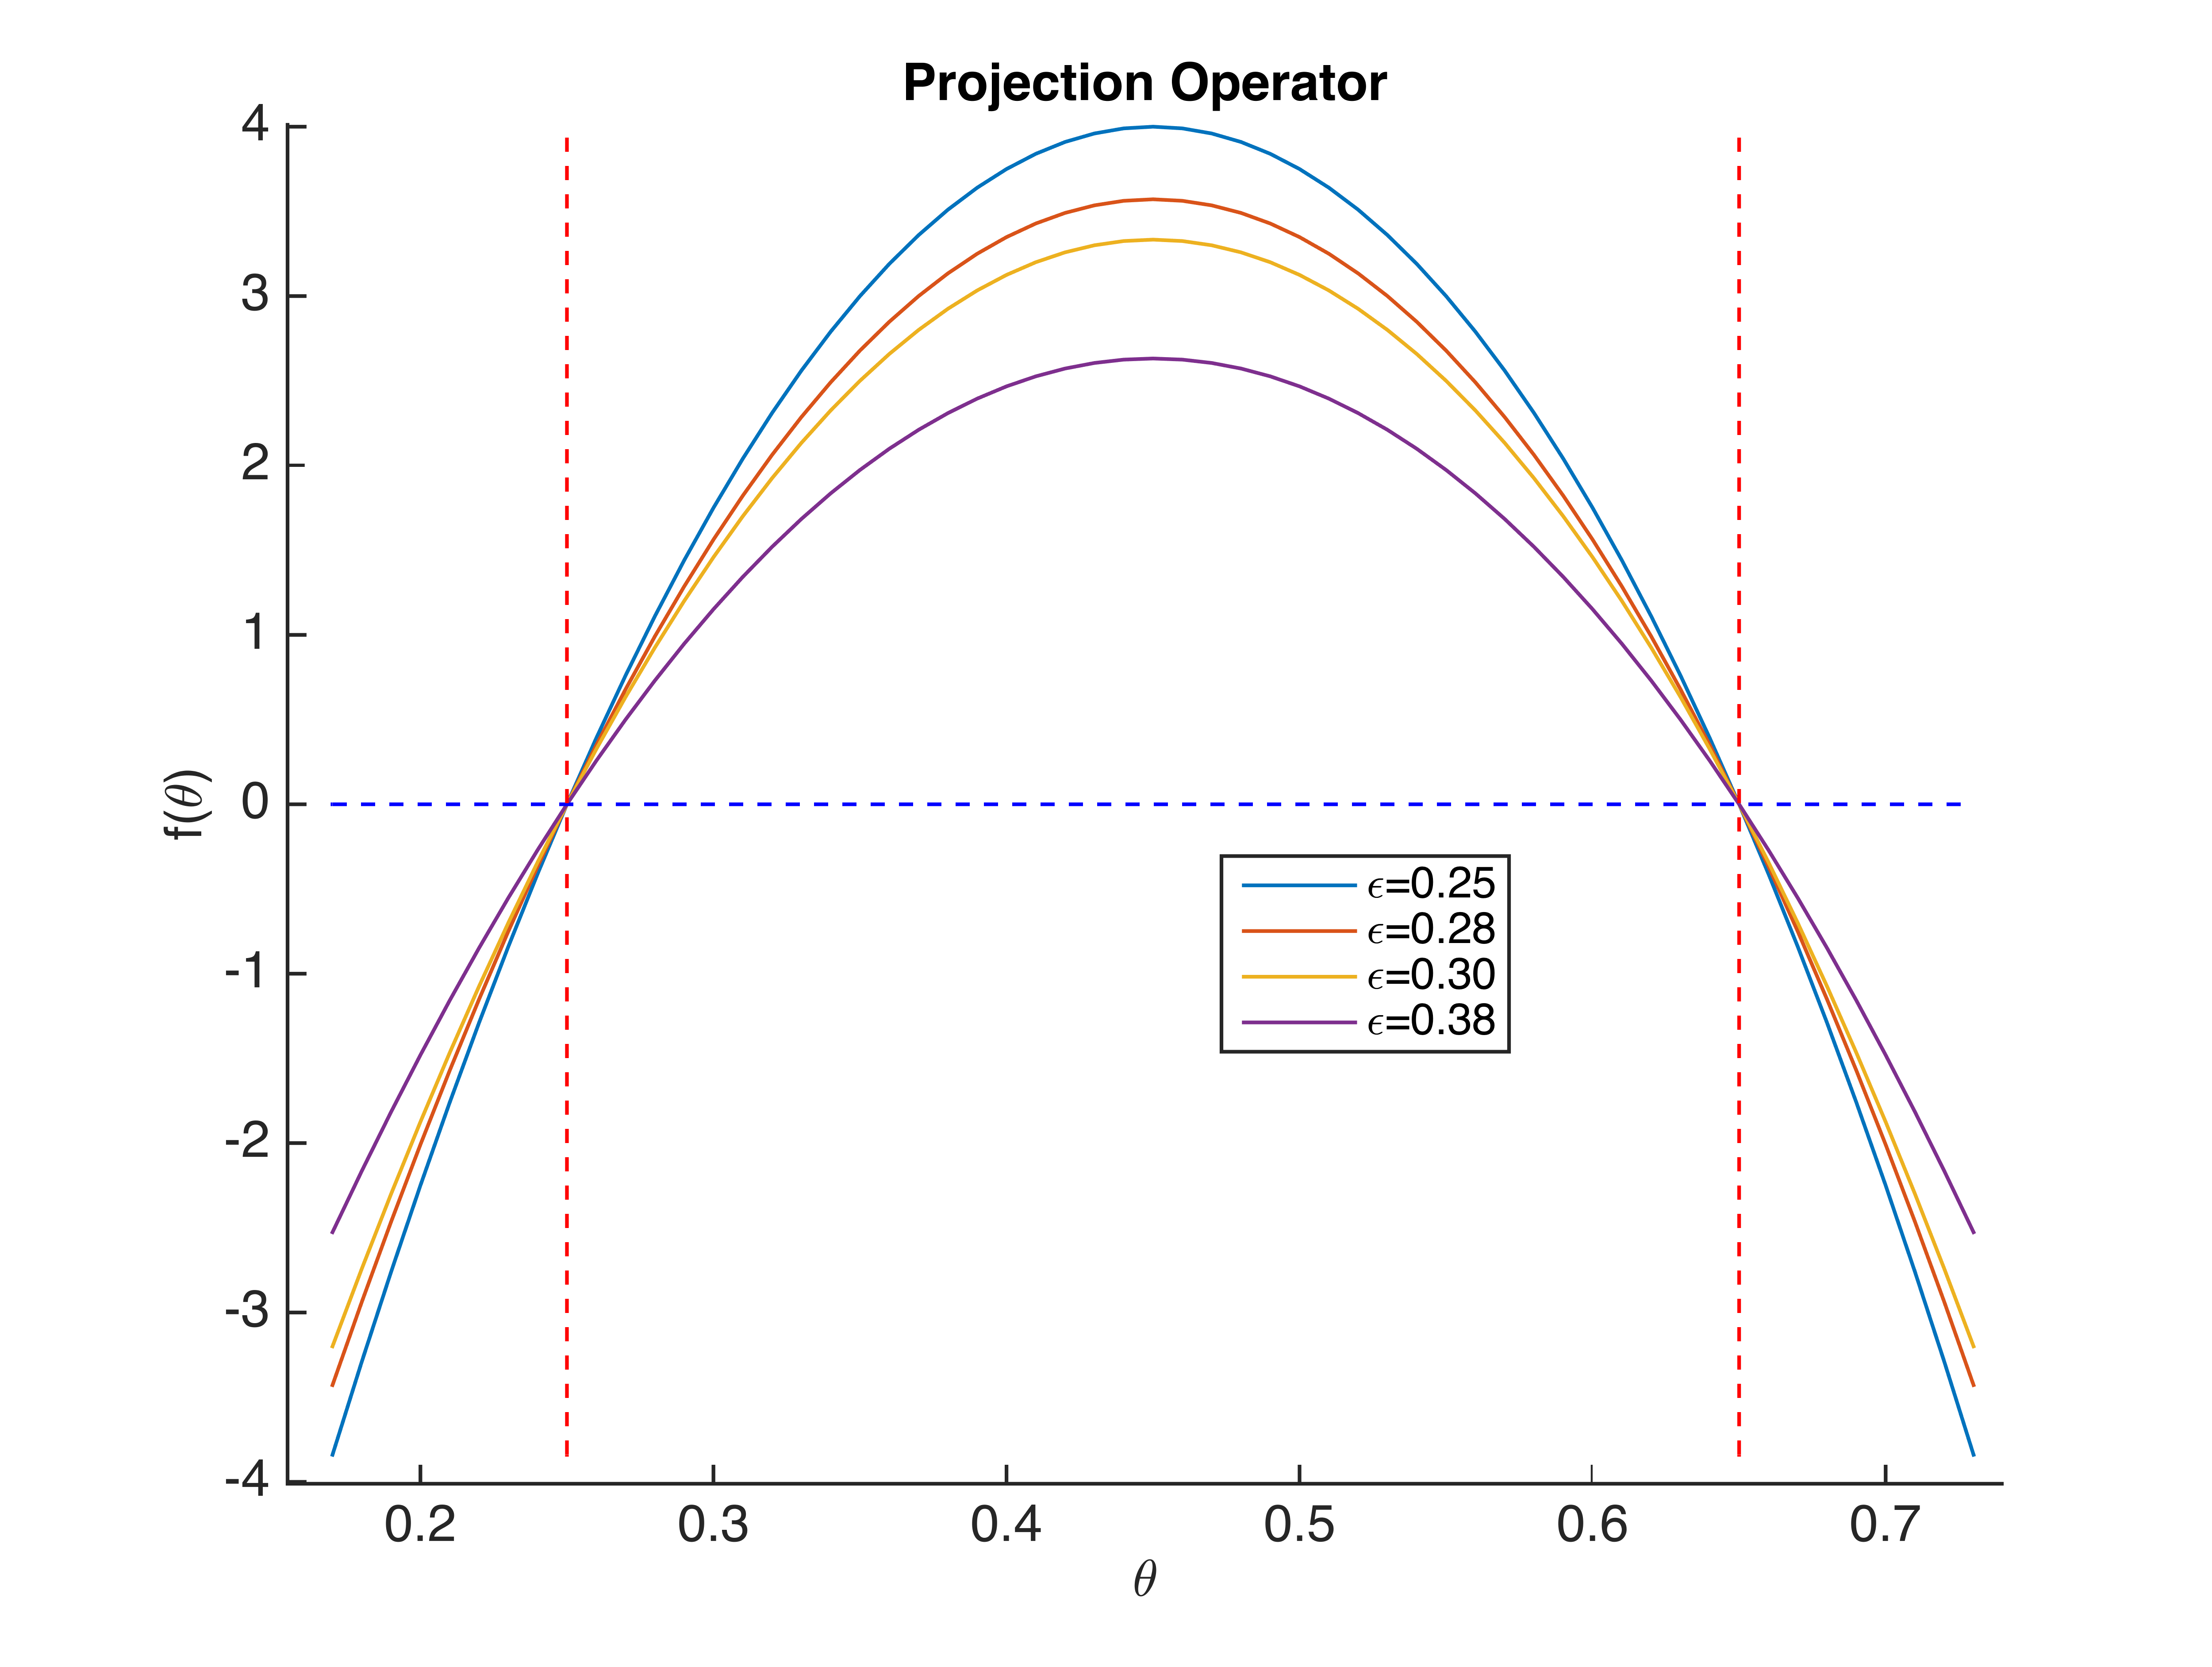
\includegraphics[width=1\textwidth]{Projection_Operator2.png}
  \caption{Projection Operator with offset limits}
  \label{fig:projection_operator_offset}
\end{figure}

\section{C++ Implementation}


\begin{lstlisting}
float projection_operator(float theta,float y,float epsilon,
float theta_max,float theta_min)
{
	
	// Calculate convex function
	float f_theta = (-4*(theta_min-theta)*(theta_max-theta))
	/(epsilon*(theta_max-theta_min)^2);
	float f_theta_dot = (4*(theta_min+theta_max-(2*theta)))
	/(epsilon*(theta_max-theta_min)^2);	

	float projection_out = y;

	if (f_theta <=0 && f_theta_dot*y < 0)
	{
		projection_out = y*(f_theta+1); // y-(y*-f_theta);
	}	
 
   	return projection_out;
}
\end{lstlisting}